\section{Padding Token [PAD]}

The padding token, denoted as \pad{}, represents one of the most fundamental yet often overlooked components in transformer architectures. While seemingly simple, the \pad{} token enables efficient batch processing and serves as a cornerstone for practical deployment of transformer models. Understanding its mechanics, implications, and optimization strategies is crucial for effective model implementation.
\begin{comment}
Feedback: This is a solid introduction. To make it even more compelling, you could frame padding as a core engineering trade-off. For example: "The [PAD] token represents a fundamental compromise between the messy, variable-length nature of real-world data and the rigid, fixed-size requirements of high-performance computing hardware. Mastering its use is key to building efficient and scalable transformer systems."
\end{comment}

\subsection{The Batching Challenge}

Transformer models process sequences of variable length, but modern deep learning frameworks require fixed-size tensors for efficient computation. This fundamental mismatch creates the need for padding:

\begin{itemize}
\item \textbf{Variable Input Lengths}: Natural text varies dramatically in length
\item \textbf{Batch Processing}: Training and inference require uniform tensor dimensions
\item \textbf{Hardware Efficiency}: GPUs perform best with regular memory access patterns
\item \textbf{Parallelization}: Fixed dimensions enable SIMD operations
\end{itemize}

The \pad{} token solves this by filling shorter sequences to match the longest sequence in each batch.

\subsection{Padding Mechanisms}

\subsubsection{Basic Padding Strategy}
For a batch of sequences with lengths $[l_1, l_2, \ldots, l_B]$, padding extends each sequence to $L = \max(l_1, l_2, \ldots, l_B)$:

$\text{sequence}_i = \{x_{i,1}, x_{i,2}, \ldots, x_{i,l_i}, \pad{}, \pad{}, \ldots, \pad{}\}$

where the number of padding tokens is $(L - l_i)$.

\subsubsection{Padding Positions}
Different strategies exist for padding placement:

\begin{itemize}
\item \textbf{Right Padding} (most common): Append \pad{} tokens to the end
\item \textbf{Left Padding}: Prepend \pad{} tokens to the beginning  
\item \textbf{Center Padding}: Distribute \pad{} tokens around the original sequence
\end{itemize}
\begin{comment}
Feedback: The distinction between left and right padding is important but not fully explained. It would be very helpful to add a sentence on the implications. For example: "While right-padding is common for encoder-only models like BERT, left-padding is often crucial for decoder-only models like GPT. This is because a decoder must not attend to future tokens, and left-padding ensures that the real content tokens maintain their correct causal positions relative to each other, which is essential for coherent text generation."
\end{comment}

\begin{lstlisting}[language=Python, caption=Padding Implementation]
import torch
from transformers import BertTokenizer

tokenizer = BertTokenizer.from_pretrained('bert-base-uncased')

# Sample texts of different lengths
texts = [
    "Hello world",
    "The quick brown fox jumps over the lazy dog",
    "AI is amazing"
]

# Tokenize and pad
inputs = tokenizer(texts, padding=True, truncation=True, 
                  return_tensors='pt', max_length=128)

print("Input IDs shape:", inputs['input_ids'].shape)
print("Attention mask shape:", inputs['attention_mask'].shape)

# Examine padding
for i, text in enumerate(texts):
    tokens = tokenizer.convert_ids_to_tokens(inputs['input_ids'][i])
    mask = inputs['attention_mask'][i]
    
    print(f"\nText {i+1}: {text}")
    print(f"Tokens: {tokens[:15]}...")  # Show first 15 tokens
    print(f"Mask:   {mask[:15].tolist()}...")
    
    # Count padding tokens
    pad_count = (inputs['input_ids'][i] == tokenizer.pad_token_id).sum()
    print(f"Padding tokens: {pad_count}")
\end{lstlisting}

\subsection{Attention Masking}

The critical challenge with padding is preventing the model from attending to meaningless \pad{} tokens. This is achieved through attention masking:

\subsubsection{Attention Mask Mechanism}
An attention mask $M \in \{0, 1\}^{B \times L}$ where:
\begin{itemize}
\item $M_{i,j} = 1$ for real tokens
\item $M_{i,j} = 0$ for padding tokens
\end{itemize}

The masked attention computation becomes:
$\text{Attention}(Q, K, V) = \text{softmax}\left(\frac{QK^T}{\sqrt{d_k}} + (1-M) \cdot (-\infty)\right)V$

Setting masked positions to $-\infty$ ensures they receive zero attention after softmax.

\subsubsection{Implementation Details}
\begin{lstlisting}[language=Python, caption=Attention Masking]
import torch
import torch.nn.functional as F

def masked_attention(query, key, value, mask):
    """
    Compute masked self-attention.
    
    Args:
        query, key, value: [batch_size, seq_len, d_model]
        mask: [batch_size, seq_len] where 1=real, 0=padding
    """
    batch_size, seq_len, d_model = query.shape
    
    # Compute attention scores
    scores = torch.matmul(query, key.transpose(-2, -1)) / (d_model ** 0.5)
    
    # Expand mask for broadcasting
    mask = mask.unsqueeze(1).expand(batch_size, seq_len, seq_len)
    
    # Apply mask (set padding positions to large negative value)
    scores = scores.masked_fill(mask == 0, -1e9)
    
    # Apply softmax
    attention_weights = F.softmax(scores, dim=-1)
    
    # Apply attention to values
    output = torch.matmul(attention_weights, value)
    
    return output, attention_weights

# Example usage
batch_size, seq_len, d_model = 2, 10, 64
query = torch.randn(batch_size, seq_len, d_model)
key = value = query  # Self-attention

# Create mask: first sequence has 7 real tokens, second has 4
mask = torch.tensor([
    [1, 1, 1, 1, 1, 1, 1, 0, 0, 0],  # 7 real tokens
    [1, 1, 1, 1, 0, 0, 0, 0, 0, 0]   # 4 real tokens
])

output, weights = masked_attention(query, key, value, mask)
print(f"Output shape: {output.shape}")
print(f"Attention weights shape: {weights.shape}")

# Verify padding positions have zero attention
print("Attention to padding positions:", weights[0, 0, 7:])  # Should be ~0
\end{lstlisting}

\subsection{Computational Implications}

\subsubsection{Memory Overhead}
Padding introduces significant memory overhead:
\begin{itemize}
\item \textbf{Wasted Computation}: Processing meaningless \pad{} tokens
\item \textbf{Memory Expansion}: Batch memory scales with longest sequence
\item \textbf{Attention Complexity}: Quadratic scaling includes padding positions
\end{itemize}

For a batch with sequence lengths $[10, 50, 100, 25]$, all sequences are padded to length 100, wasting:
$\text{Wasted positions} = 4 \times 100 - (10 + 50 + 100 + 25) = 215 \text{ positions}$

\subsubsection{Efficiency Optimizations}
Several strategies mitigate padding overhead:

\begin{itemize}
\item \textbf{Dynamic Batching}: Group sequences of similar lengths
\item \textbf{Bucketing}: Pre-sort sequences by length for batching
\item \textbf{Packed Sequences}: Remove padding and use position offsets
\item \textbf{Variable-Length Attention}: Sparse attention patterns
\end{itemize}

\begin{figure}[h]
\centering
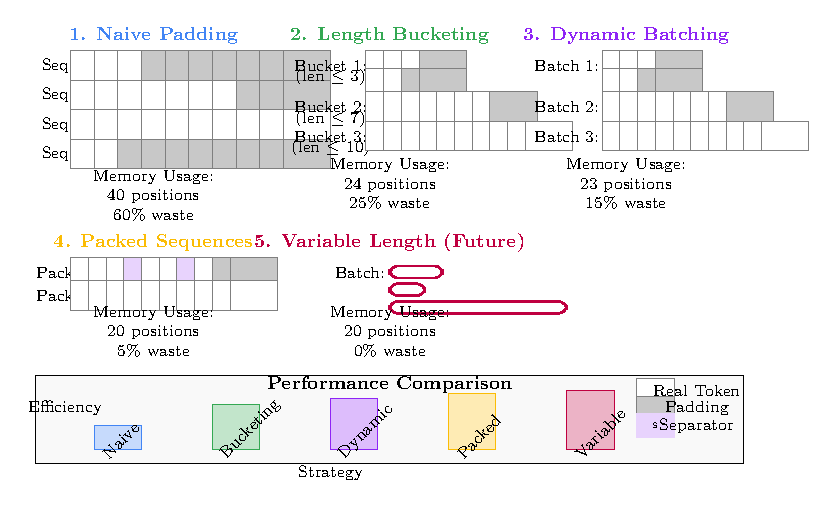
\includegraphics[width=0.95\textwidth]{part1/chapter02/fig_padding_strategies.pdf}
\caption{Comparison of padding strategies and their memory efficiency}
\end{figure}

\subsection{Training Considerations}

\subsubsection{Loss Computation}
When computing loss, padding positions must be excluded:

\begin{lstlisting}[language=Python, caption=Masked Loss Computation]
import torch
import torch.nn as nn

def compute_masked_loss(predictions, targets, mask):
    """
    Compute loss only on non-padding positions.
    
    Args:
        predictions: [batch_size, seq_len, vocab_size]
        targets: [batch_size, seq_len]
        mask: [batch_size, seq_len] where 1=real, 0=padding
    """
    # Flatten for loss computation
    predictions_flat = predictions.view(-1, predictions.size(-1))
    targets_flat = targets.view(-1)
    mask_flat = mask.view(-1)
    
    # Compute loss
    loss_fn = nn.CrossEntropyLoss(reduction='none')
    losses = loss_fn(predictions_flat, targets_flat)
    
    # Apply mask and compute mean over valid positions
    masked_losses = losses * mask_flat
    total_loss = masked_losses.sum() / mask_flat.sum()
    
    return total_loss

# Example usage
batch_size, seq_len, vocab_size = 2, 10, 30000
predictions = torch.randn(batch_size, seq_len, vocab_size)
targets = torch.randint(0, vocab_size, (batch_size, seq_len))
mask = torch.tensor([
    [1, 1, 1, 1, 1, 1, 1, 0, 0, 0],
    [1, 1, 1, 1, 0, 0, 0, 0, 0, 0]
])

loss = compute_masked_loss(predictions, targets, mask)
print(f"Masked loss: {loss.item():.4f}")
\end{lstlisting}

\subsubsection{Gradient Flow}
Proper masking ensures gradients don't flow through padding positions:
\begin{itemize}
\item \textbf{Forward Pass}: Padding tokens receive zero attention
\item \textbf{Backward Pass}: Zero gradients for padding token embeddings
\item \textbf{Optimization}: Padding embeddings remain unchanged during training
\end{itemize}

\subsection{Advanced Padding Strategies}

\subsubsection{Dynamic Padding}
Instead of static maximum length, adapt padding to each batch:

\begin{lstlisting}[language=Python]
def dynamic_batch_padding(sequences, tokenizer):
    """Create batches with minimal padding."""
    # Sort by length for efficient batching
    sorted_sequences = sorted(sequences, key=len)
    
    batches = []
    current_batch = []
    current_max_len = 0
    
    for seq in sorted_sequences:
        if not current_batch or len(seq) <= current_max_len * 1.2:  # 20% tolerance
            current_batch.append(seq)
            current_max_len = max(current_max_len, len(seq))
        else:
            # Process current batch
            if current_batch:
                batches.append(pad_batch(current_batch, tokenizer))
            current_batch = [seq]
            current_max_len = len(seq)
    
    # Process final batch
    if current_batch:
        batches.append(pad_batch(current_batch, tokenizer))
    
    return batches

def pad_batch(sequences, tokenizer):
    """Pad a batch to the longest sequence in the batch."""
    max_len = max(len(seq) for seq in sequences)
    
    padded_sequences = []
    attention_masks = []
    
    for seq in sequences:
        padding_length = max_len - len(seq)
        padded_seq = seq + [tokenizer.pad_token_id] * padding_length
        attention_mask = [1] * len(seq) + [0] * padding_length
        
        padded_sequences.append(padded_seq)
        attention_masks.append(attention_mask)
    
    return {
        'input_ids': torch.tensor(padded_sequences),
        'attention_mask': torch.tensor(attention_masks)
    }
\end{lstlisting}

\subsubsection{Packed Sequences}
For maximum efficiency, some implementations pack multiple sequences without padding:

\begin{lstlisting}[language=Python]
def pack_sequences(sequences, max_length=512):
    """Pack multiple sequences into fixed-length chunks."""
    packed_sequences = []
    current_sequence = []
    current_length = 0
    
    for seq in sequences:
        if current_length + len(seq) + 1 <= max_length:  # +1 for separator
            if current_sequence:
                current_sequence.append(tokenizer.sep_token_id)
                current_length += 1
            current_sequence.extend(seq)
            current_length += len(seq)
        else:
            # Pad current sequence and start new one
            if current_sequence:
                padding = [tokenizer.pad_token_id] * (max_length - current_length)
                packed_sequences.append(current_sequence + padding)
            
            current_sequence = seq
            current_length = len(seq)
    
    # Handle final sequence
    if current_sequence:
        padding = [tokenizer.pad_token_id] * (max_length - current_length)
        packed_sequences.append(current_sequence + padding)
    
    return packed_sequences
\end{lstlisting}

\subsection{Padding in Different Model Architectures}

\subsubsection{Encoder Models (BERT-style)}
\begin{itemize}
\item Bidirectional attention requires careful masking
\item Padding typically added at the end
\item Special tokens (\cls{}, \sep{}) not affected by padding
\end{itemize}

\subsubsection{Decoder Models (GPT-style)}
\begin{itemize}
\item Causal masking combined with padding masking
\item Left-padding often preferred to maintain causal structure
\item Generation requires dynamic padding handling
\end{itemize}

\subsubsection{Encoder-Decoder Models (T5-style)}
\begin{itemize}
\item Separate padding for encoder and decoder sequences
\item Cross-attention masking between encoder and decoder
\item Complex masking patterns for sequence-to-sequence tasks
\end{itemize}

\subsection{Performance Optimization}

\subsubsection{Hardware-Specific Considerations}
\begin{itemize}
\item \textbf{GPU Memory}: Minimize padding to fit larger batches
\item \textbf{Tensor Cores}: Some padding may improve hardware utilization
\item \textbf{Memory Bandwidth}: Reduce data movement through efficient padding
\end{itemize}

\subsubsection{Adaptive Strategies}
Modern frameworks implement adaptive padding:
\begin{itemize}
\item Monitor padding overhead per batch
\item Adjust batching strategy based on sequence length distribution
\item Use dynamic attention patterns for long sequences
\end{itemize}

\subsection{Common Pitfalls and Solutions}

\subsubsection{Incorrect Masking}
\textbf{Problem}: Forgetting to mask padding positions in attention
\textbf{Solution}: Always verify attention mask implementation
\begin{comment}
Feedback: To make this pitfall more impactful, describe the consequence. For example: "Consequence: The model's attention is diluted by attending to meaningless padding tokens, leading to degraded performance and nonsensical representations."
\end{comment}

\subsubsection{Loss Computation Errors}
\textbf{Problem}: Including padding positions in loss calculation
\textbf{Solution}: Implement proper masked loss functions
\begin{comment}
Feedback: Similarly, what is the consequence? "Consequence: The model is penalized for its predictions on padding tokens, which can destabilize training and lead to the model learning to simply predict padding."
\end{comment}

\subsubsection{Memory Inefficiency}
\textbf{Problem}: Excessive padding leading to OOM errors
\textbf{Solution}: Implement dynamic batching and length bucketing

\subsubsection{Inconsistent Padding}
\textbf{Problem}: Different padding strategies between training and inference
\textbf{Solution}: Standardize padding approach across all phases

\subsection{Future Developments}

\subsubsection{Dynamic Attention}
Emerging techniques eliminate the need for padding:
\begin{itemize}
\item Flash Attention for variable-length sequences
\item Block-sparse attention patterns
\item Adaptive sequence processing
\end{itemize}

\subsubsection{Hardware Improvements}
Next-generation hardware may reduce padding overhead:
\begin{itemize}
\item Variable-length tensor support
\item Efficient irregular memory access
\item Specialized attention accelerators
\end{itemize}

\begin{principle}[Padding Best Practices]
\begin{enumerate}
\item \textbf{Minimize Overhead}: Use dynamic batching and length bucketing
\item \textbf{Correct Masking}: Always implement proper attention masking
\item \textbf{Efficient Loss}: Exclude padding positions from loss computation
\item \textbf{Memory Management}: Monitor and optimize memory usage
\item \textbf{Consistency}: Maintain identical padding strategies across training and inference
\end{enumerate}
\end{principle}
\begin{comment}
Feedback: This list can be made more actionable. For "Minimize Overhead," you could add: "Before training, analyze the length distribution of your dataset. If it is highly skewed, implementing length-based bucketing is one of the highest-impact optimizations you can make." For "Consistency," you could suggest: "Encapsulate your tokenization and padding logic in a single, version-controlled function or class that is used by both your training and inference pipelines to prevent subtle bugs."
\end{comment}

The \pad{} token, while conceptually simple, requires careful implementation to achieve efficient and correct transformer behavior. Understanding its implications for memory usage, computation, and model training is essential for building scalable transformer-based systems. As the field moves toward more efficient architectures, the role of padding continues to evolve, but its fundamental importance in enabling batch processing remains central to practical transformer deployment.